\documentclass[12pt,a4paper]{article}
\usepackage{amsmath,amssymb,mathrsfs,tikz,times,pifont}
\usepackage{enumitem}
\newcommand\circitem[1]{%
\tikz[baseline=(char.base)]{
\node[circle,draw=gray, fill=red!55,
minimum size=1.2em,inner sep=0] (char) {#1};}}
\newcommand\boxitem[1]{%
\tikz[baseline=(char.base)]{
\node[fill=cyan,
minimum size=1.2em,inner sep=0] (char) {#1};}}
\setlist[enumerate,1]{label=\protect\circitem{\arabic*}}
\setlist[enumerate,2]{label=\protect\boxitem{\alph*}}
%%%::::::by chnini ameur :::::::%%%
\everymath{\displaystyle}
\usepackage[left=1cm,right=1cm,top=1cm,bottom=1.7cm]{geometry}
\usepackage[colorlinks=true, linkcolor=blue, urlcolor=blue, citecolor=blue]{hyperref}
\usepackage{array,multirow}
\usepackage[most]{tcolorbox}
\usepackage{varwidth}
\usepackage{float} %pour utiliser l'option [H] qui force l'image à apparaître exactement à l'endroit où elle est placée dans le code.
\tcbuselibrary{skins,hooks}
\usetikzlibrary{patterns}
%%%::::::by chnini ameur :::::::%%%
\newtcolorbox{exa}[2][]{enhanced,breakable,before skip=2mm,after skip=5mm,
colback=yellow!20!white,colframe=black!20!blue,boxrule=0.5mm,
attach boxed title to top left ={xshift=0.6cm,yshift*=1mm-\tcboxedtitleheight},
fonttitle=\bfseries,
title={#2},#1,
% varwidth boxed title*=-3cm,
boxed title style={frame code={
\path[fill=tcbcolback!30!black]
([yshift=-1mm,xshift=-1mm]frame.north west)
arc[start angle=0,end angle=180,radius=1mm]
([yshift=-1mm,xshift=1mm]frame.north east)
arc[start angle=180,end angle=0,radius=1mm];
\path[left color=tcbcolback!60!black,right color = tcbcolback!60!black,
middle color = tcbcolback!80!black]
([xshift=-2mm]frame.north west) -- ([xshift=2mm]frame.north east)
[rounded corners=1mm]-- ([xshift=1mm,yshift=-1mm]frame.north east)
-- (frame.south east) -- (frame.south west)
-- ([xshift=-1mm,yshift=-1mm]frame.north west)
[sharp corners]-- cycle;
},interior engine=empty,
},interior style={top color=yellow!5}}
%%%%%%%%%%%%%%%%%%%%%%%

\usepackage{fancyhdr}
\usepackage{eso-pic}         % Pour ajouter des éléments en arrière-plan
% Commande pour ajouter du texte en arrière-plan
\usepackage{tkz-tab}
\AddToShipoutPicture{
    \AtTextCenter{%
        \makebox[0pt]{\rotatebox{80}{\textcolor[gray]{0.7}{\fontsize{5cm}{5cm}\selectfont PGB}}}
    }
}
\usepackage{lastpage}
\fancyhf{}
\pagestyle{fancy}
\renewcommand{\footrulewidth}{1pt}
\renewcommand{\headrulewidth}{0pt}
\renewcommand{\footruleskip}{10pt}
\fancyfoot[R]{
\color{blue}\ding{45}\ \textbf{2024}
}
\fancyfoot[L]{
\color{blue}\ding{45}\ \textbf{Prof:M. BA}
}
\cfoot{\bf
\thepage /
\pageref{LastPage}}

% Définition de l'encadré adaptatif avec fond jaune
\newtcolorbox{resultbox}{
    colback=red!30, % Fond rouge clair
    colframe=black, % Bordure noire fine
    sharp corners, % Coins nets
    boxrule=0.5pt, % Contour léger
    boxsep=2pt, % Espacement interne
    left=5pt, right=5pt, top=2pt, bottom=2pt, % Marges internes
}

\begin{document}
\renewcommand{\arraystretch}{1.5}
\renewcommand{\arrayrulewidth}{1.2pt}
\begin{tikzpicture}[overlay,remember picture]
\node[draw=blue,line width=1.2pt,fill=purple,text=blue,inner sep=3mm,rounded corners,pattern=dots]at ([yshift=-2.5cm]current page.north) {\begingroup\setlength{\fboxsep}{0pt}\colorbox{white}{\begin{tabular}{|*1{>{\centering \arraybackslash}p{0.28\textwidth}} |*2{>{\centering \arraybackslash}p{0.2\textwidth}|} *1{>{\centering \arraybackslash}p{0.19\textwidth}|} }
\hline
\multicolumn{3}{|c|}{$\diamond$$\diamond$$\diamond$\ \textbf{Lycée de Dindéfélo}\ $\diamond$$\diamond$$\diamond$ }& \textbf{A.S. : 2024/2025} \\ \hline
\textbf{Matière: Mathématiques}& \textbf{Niveau : T}\textbf{S2} &\textbf{Date: 09/12/2024} & \textbf{Durée : 4 heures} \\ \hline
\multicolumn{4}{|c|}{\parbox[c]{10cm}{\begin{center}
\textbf{{\Large\sffamily Correction du devoir n$ ^{\circ} $ 1 Du 1$ ^\text{\bf er} $ Semestre}}
\end{center}}} \\ \hline
\end{tabular}}\endgroup};
\end{tikzpicture}
\vspace{3cm}

\section*{\underline{Exercice 2 :} 2,25 points }
Déterminons les limites suivantes :

\(\textbf{1.} \lim\limits_{x \to +\infty} \ln\left[ \frac{x+1}{x^2 + x + 1}\right]  \quad \)

\(
\begin{aligned}
    \lim\limits_{x \to +\infty} \ln\left[ \frac{x+1}{x^2 + x + 1}\right]:
    \begin{cases}
        \lim\limits_{x \to +\infty} \frac{x+1}{x^2 + x + 1}=0 \\
        \lim\limits_{x \to 0}\ln(x)=-\infty
    \end{cases}\text{Par composition, }\lim\limits_{x \to +\infty} \ln\left[ \frac{x+1}{x^2 + x + 1}\right]=-\infty
\end{aligned}
\)

\begin{resultbox}
    \[
        \mathbf{\ln\left[ \frac{x+1}{x^2 + x + 1}\right]=-\infty}
    \]
\end{resultbox}

\( \textbf{2.} \lim\limits_{x \to +\infty} \frac{\ln(x+2)}{\ln(x+1)} \)

\(
\begin{aligned}
    \lim\limits_{x \to +\infty} \frac{\ln(x+2)}{\ln(x+1)} & = \lim\limits_{x \to +\infty} \frac{\ln\left[x\left( 1+ \frac{2}{x}\right) \right]}{\ln\left[x\left( 1+ \frac{1}{x}\right) \right]}                                                      \\
                                                          & = \lim\limits_{x \to +\infty} \frac{ \ln(x) + \ln\left( 1+ \frac{2}{x}\right) }{ \ln(x) + \ln\left( 1+ \frac{1}{x}\right)}                                                               \\
                                                          & = \lim\limits_{x \to +\infty} \frac{ \ln(x) \left[ 1+ \frac{\ln\left( 1+ \frac{2}{x}\right)}{\ln(x)} \right] }{ \ln(x) \left[ 1+ \frac{\ln\left( 1+ \frac{1}{x}\right)}{\ln(x)} \right]} \\
                                                          & = \lim\limits_{x \to +\infty} \frac{ \left[ 1+ \frac{\ln\left( 1+ \frac{2}{x}\right)}{\ln(x)} \right] }{ \left[1+ \frac{\ln\left( 1+ \frac{1}{x}\right)}{\ln(x)} \right]}                \\
                                                          & = 1                                                                                                                                                                                      \\
\end{aligned}\\
\)

\begin{resultbox}
    \[
        \mathbf{\lim\limits_{x \to +\infty} \frac{\ln(x+2)}{\ln(x+1)}=1}
    \]
\end{resultbox}

\( \textbf{3.} \lim\limits_{x \to 0^+} \frac{\ln x+2}{\ln x+1} \)

\(
\begin{aligned}
    \lim\limits_{x \to 0^+} \frac{\ln x+2}{\ln x+1} & =\lim\limits_{x \to 0^+} \frac{\ln x\left(1+\frac{2}{\ln x}\right)}{\ln x\left(1+\frac{1}{\ln x}\right)} \\
    =                                               & \lim\limits_{x \to 0^+} \frac{\left(1+\frac{2}{\ln x}\right)}{\left(1+\frac{1}{\ln x}\right)}            \\
    =                                               & 1
\end{aligned}
\)

\begin{resultbox}
    \[
        \mathbf{\lim\limits_{x \to +\infty} \lim\limits_{x \to 0^+} \frac{\ln x+2}{\ln x+1}=1}
    \]
\end{resultbox}

\(
\textbf{4.} \lim\limits_{x \to +\infty} \frac{\ln x}{\sqrt{x}}
\)

\(
\begin{aligned}
    \lim\limits_{x \to +\infty} \frac{\ln x}{\sqrt{x}} & =\lim\limits_{x \to +\infty} \frac{\ln\left[(\sqrt{x})^{2}\right] }{\sqrt{x}} \\
                                                       & =\lim\limits_{x \to +\infty} \frac{2\ln\left[\sqrt{x}\right] }{\sqrt{x}}      \\
                                                       & =0                                                                            \\
\end{aligned}
\)

\begin{resultbox}
    \[
        \mathbf{\lim\limits_{x \to +\infty} \frac{\ln x}{\sqrt{x}}=0}
    \]
\end{resultbox}

\section*{\underline{Problème :} 11,75 points }
\subsection*{\underline{\textbf{Partie A}}:\textbf{ 2,75 pts}}

Soit \( g(x) = 2x \ln(-x) + x + 1 \).

\begin{enumerate}
    \item Déterminons l’ensemble de définition \( D_g \) de \( g \).\hfill \textbf{(0,5 pt)}

          \(g\) existe ssi \(-x>0\)

          \(\begin{aligned}
              -x>0 & \implies x<0              \\
                   & \implies x\in ]-\infty;0[
          \end{aligned}\)

          Donc \(Dg=]-\infty;0[\)

          \begin{resultbox}
              \[
                  \mathbf{Dg=]-\infty;0[}
              \]
          \end{resultbox}

    \item Calculons les limites aux bornes de \( D_g \).\hfill \textbf{(0,5 pt)}

          \underline{En $-\infty$}

          \( \begin{aligned}
              \lim\limits_{x\to -\infty}g(x) & =\lim\limits_{x\to -\infty} 2x \ln(-x) + x + 1 \\
                                             & =-\infty
          \end{aligned} \)

          \( \lim\limits_{x\to -\infty}g(x) = -\infty \)

          \begin{resultbox}
              \[
                  \mathbf{\lim\limits_{x\to -\infty}g(x) = -\infty}
              \]
          \end{resultbox}

          \underline{En $0^{-}$}

          \( \begin{aligned}
              \lim\limits_{x\to 0^{-}}g(x) & =\lim\limits_{x\to 0^{-}} 2x \ln(-x) + x + 1     \\
                                           & =\lim\limits_{x\to 0^{-}} -2(-x \ln(-x)) + x + 1 \\
                                           & =1
          \end{aligned} \)

          \( \lim\limits_{x\to 0^{-}}g(x) = 1 \)

          \begin{resultbox}
              \[
                  \mathbf{\lim\limits_{x\to 0^{-}}g(x) = 1}
              \]
          \end{resultbox}
    \item Étudions les variations de \( g \).\hfill \textbf{(1 pt)}

          \(
          \begin{aligned}
              g(x) & = 2x \ln(-x) + x + 1                                  \\
                   & = 2(x \ln(-x))' + (x + 1)'                            \\
                   & = 2\left[(x)'\ln(-x)+x(\ln(-x))'\right] + 1           \\
                   & = 2\left[\ln(-x)+x\left(\frac{1}{x}\right)\right] + 1 \\
                   & = 2\left[\ln(-x)+1\right] + 1                         \\
                   & = 2\ln(-x)+ 3
          \end{aligned}
          \)
          
          \begin{resultbox}
              \[
                  \mathbf{g'(x)=2\ln(-x)+ 3}
              \]
          \end{resultbox}

          Etudions le signe de \(g\)

          Supposons que \( 2\ln(-x)+ 3 > 0 \)

          \(
          \begin{aligned}
              2\ln(-x)+ 3 > 0 & \implies \ln(-x)> \frac{-3}{2}                       \\
                              & \implies \ln(-x)> \ln\left(e^{\frac{-3}{2}}\right)   \\
                              & \implies -x> e^{\frac{-3}{2}}                        \\
                              & \implies x< -e^{\frac{-3}{2}}                        \\
                              & \implies x\in \left]-\infty;-e^{\frac{-3}{2}}\right[ \\
          \end{aligned}
          \)

          \(
            \begin{cases}
              \forall x \in \left]-\infty;-e^{\frac{-3}{2}}\right[, g'(x)>0  \text{ donc $g$ y est croissant}\\
              \forall x \in \left]-e^{\frac{-3}{2}};0\right[, g'(x)<0 \text{ donc $g$ y est décroissant}      
          \end{cases} 
          \)

                    \begin{center}
                        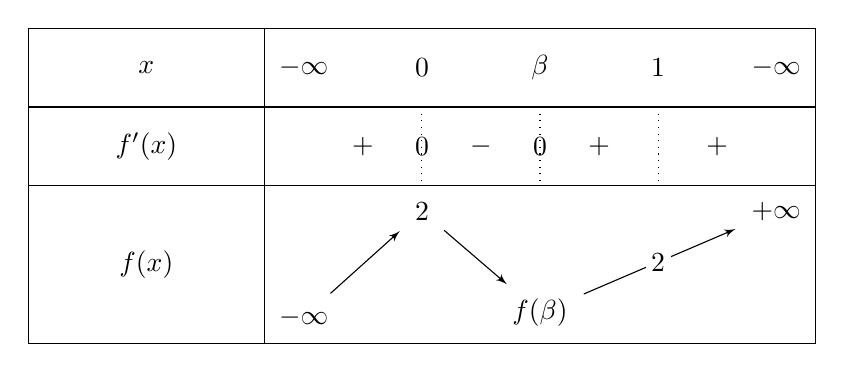
\begin{tikzpicture}
                            \tkzTabInit[lgt=3,espcl=1.5]
                            {$x$ / 1 , $f'(x)$ / 1, $f(x)$ / 2 }
                            {$-\infty$, $0$, $\beta$, 1, $-\infty$}
                            \tkzTabLine
                            {, +, z ,  -  , z , + ,t,+,}
                            \tkzTabVar
                            { -/$-\infty$ , +/$2$, -/$f(\beta)$, R/, +/$+\infty$}
                            \tkzTabIma{3}{5}{4}{2}
                        \end{tikzpicture}
                    \end{center}
        
          %\item Calculer \( g(-1) \) puis en déduire le signe de \( g(x) \).\hfill \textbf{(0,75 pt)}
\end{enumerate}

\end{document}
